\Exercise[title={Volum esfera}]
%\begin{Exercise}[label=Ex7]

  Calcula el volum d'una esfera de radi $a$ usant una integral triple.

%\end{Exercise}

\Answer

El volum de l'esfera ve donat per l'expressió:

\[
  V=\int\int\int_{\Omega} dV 
\]



Si explorem el problema usant coordenades cartesianes, l'element de volum és $\dif V= \dif x \dif y \dif z$ i els límits d'integració quedarien com:

\[
  V=\int_{-a}^a  \int_{-\sqrt{a^2-x^2}}^{\sqrt{a^2-x^2}} \int_{-\sqrt{a^2-x^2-y^2}}^{\sqrt{a^2-x^2-y^2}} \dif z \dif y \dif x 
\]

Alternativament, podem observar que la simetria de l'objecte ens permet usar coordenades esfèriques:

\begin{center}
  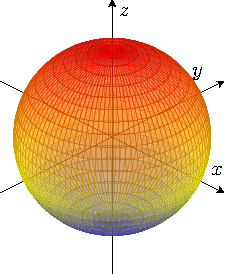
\includegraphics[width=0.3\linewidth]{sphere.pdf}
  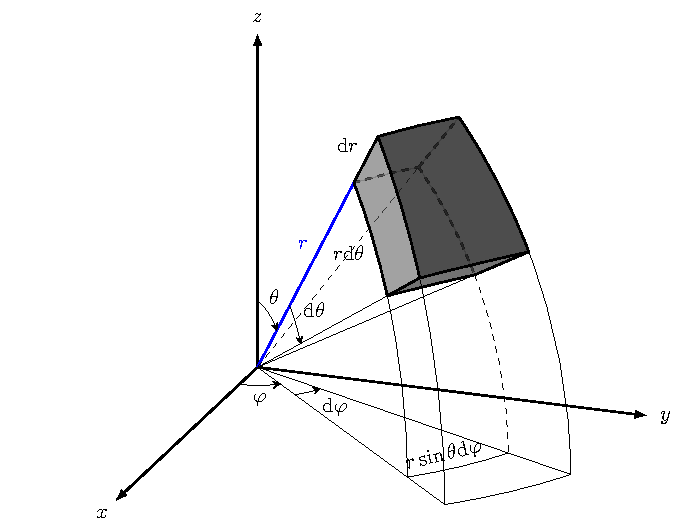
\includegraphics[width=0.6\linewidth]{CoordinatesSpherical.pdf}
\end{center}

Ara l'element de volum vindrà donat per $\dif V = r^2 \sin{\theta} \dif r \dif \theta \dif \varphi$ i els límits d'integració canviaran de forma molt favorable, ja que:

\[
\begin{cases}
  -a \leq x \leq a\\
  -\sqrt{a^2-x^2} \leq y \leq \sqrt{a^2-x^2} \\
  0 \leq z \leq a^2-x^2 - y^2\\
\end{cases}  
\Rightarrow
\begin{cases}
  0 \leq \theta \leq \pi\\
  0 \leq r \leq a \\
  0 \leq \varphi \leq 2\pi\\
\end{cases}  
\]

Així:

\begin{eqnarray*}
  V&=&\int_{0}^{2\pi}  \int_{0}^{\pi} \int_0^{a} r^2 \sin{\theta} \dif r \dif \theta \dif \varphi = \int_{0}^{2\pi} \dif \varphi  \int_{0}^{\pi} \sin{\theta} \dif \theta \int_0^{a} r^2  \dif r   \\
  &=& [\varphi]_0^{2\pi} \left[-\cos{\theta}\right]_0^{\pi} \left[\frac{r^3}{3}\right]_0^a =\boxed{\frac{4}{3}\pi a^3}
\end{eqnarray*}

%\end{Answer}
